\chapter{Probas}

As probas que detallaremos a continuación buscan identificar posibles fallos ou funcionamentos inadecuados do sistema, para garantir que este funciona de forma óptima. Así, conseguiremos o
obxectivo de ter un sistema robusto e fiable.

\section{Probas unitarias}\label{unitarias}
As probas unitarias son de vital importancia para comprobar o correcto funcionamento do código a nivel de funcións ou métodos. Estas probas consisten en comprobar compoñentes individualmente,
garantindo que funcionan de maneira axeitada.

Estas probas unitarias fixéronse de maneira manual, comprobando as diferentes funcións de extracción e transformación de datos. Comprobouse, por exemplo, o funcionamento da función de descarga de
datos, revisando que a mesma devolve os datos no formato agardado (arquivos netCDF) e que, en caso de producirse un erro na descarga, o programa pode continuar descargando o resto de arquivos
correctamente, minimizando a perda de datos. Así, se a descarga é satisfactoria, mostraranse os nomes dos arquivos que se descargaron.

Tamén se realizaron probas sobre as funcións que importan e transforman os arquivos a datos agregados de nivel L3. Neste caso, comprobouse que a función importa correctamente os arquivos, e que os
transforma empregando as operacións definidas, producindo o arquivo resultante tamén en formato netCDF e co patrón de nome desexado.

Unha vez que se implementou o servidor ERDDAP, tamén se realizaron probas sobre o mesmo, para comprobar que todo estivera en orde. Xa que o servidor se implementou de forma incremental, engadindo
os diferentes datasets e arquivos paulatinamente, puidemos comprobar non só o funcionamento do servidor en si, senón tamén que, conforme se xeraban novos arquivos, estes aparecían dispoñibles no
servidor tras o período de tempo que determinamos en \ref{erddapconf}. O servidor ERDDAP tamén dispón da súa propia interface, a cal é accesible en \url{http://13.53.65.240:8080/erddap/index.html}.
Ó acceder á mesma, preséntasenos a pantalla que se amosa na figura \ref{fig:erddap}. Nela, móstrase unha mensaxe co número de datasets dispoñibles, sobre a cal podemos facer clic para ver unha lista
cos mesmos, como a que se ve na figura \ref{fig:listaDatasets}. Dentro desta lista, premendo en \texttt{files}, poderemos ver a pantalla da figura \ref{fig:datasetCO} que mostra, para o dataset de
monóxido de carbono, os arquivos dispoñibles no mesmo, así como a información sobre o propio dataset

\begin{figure}
    \centerline{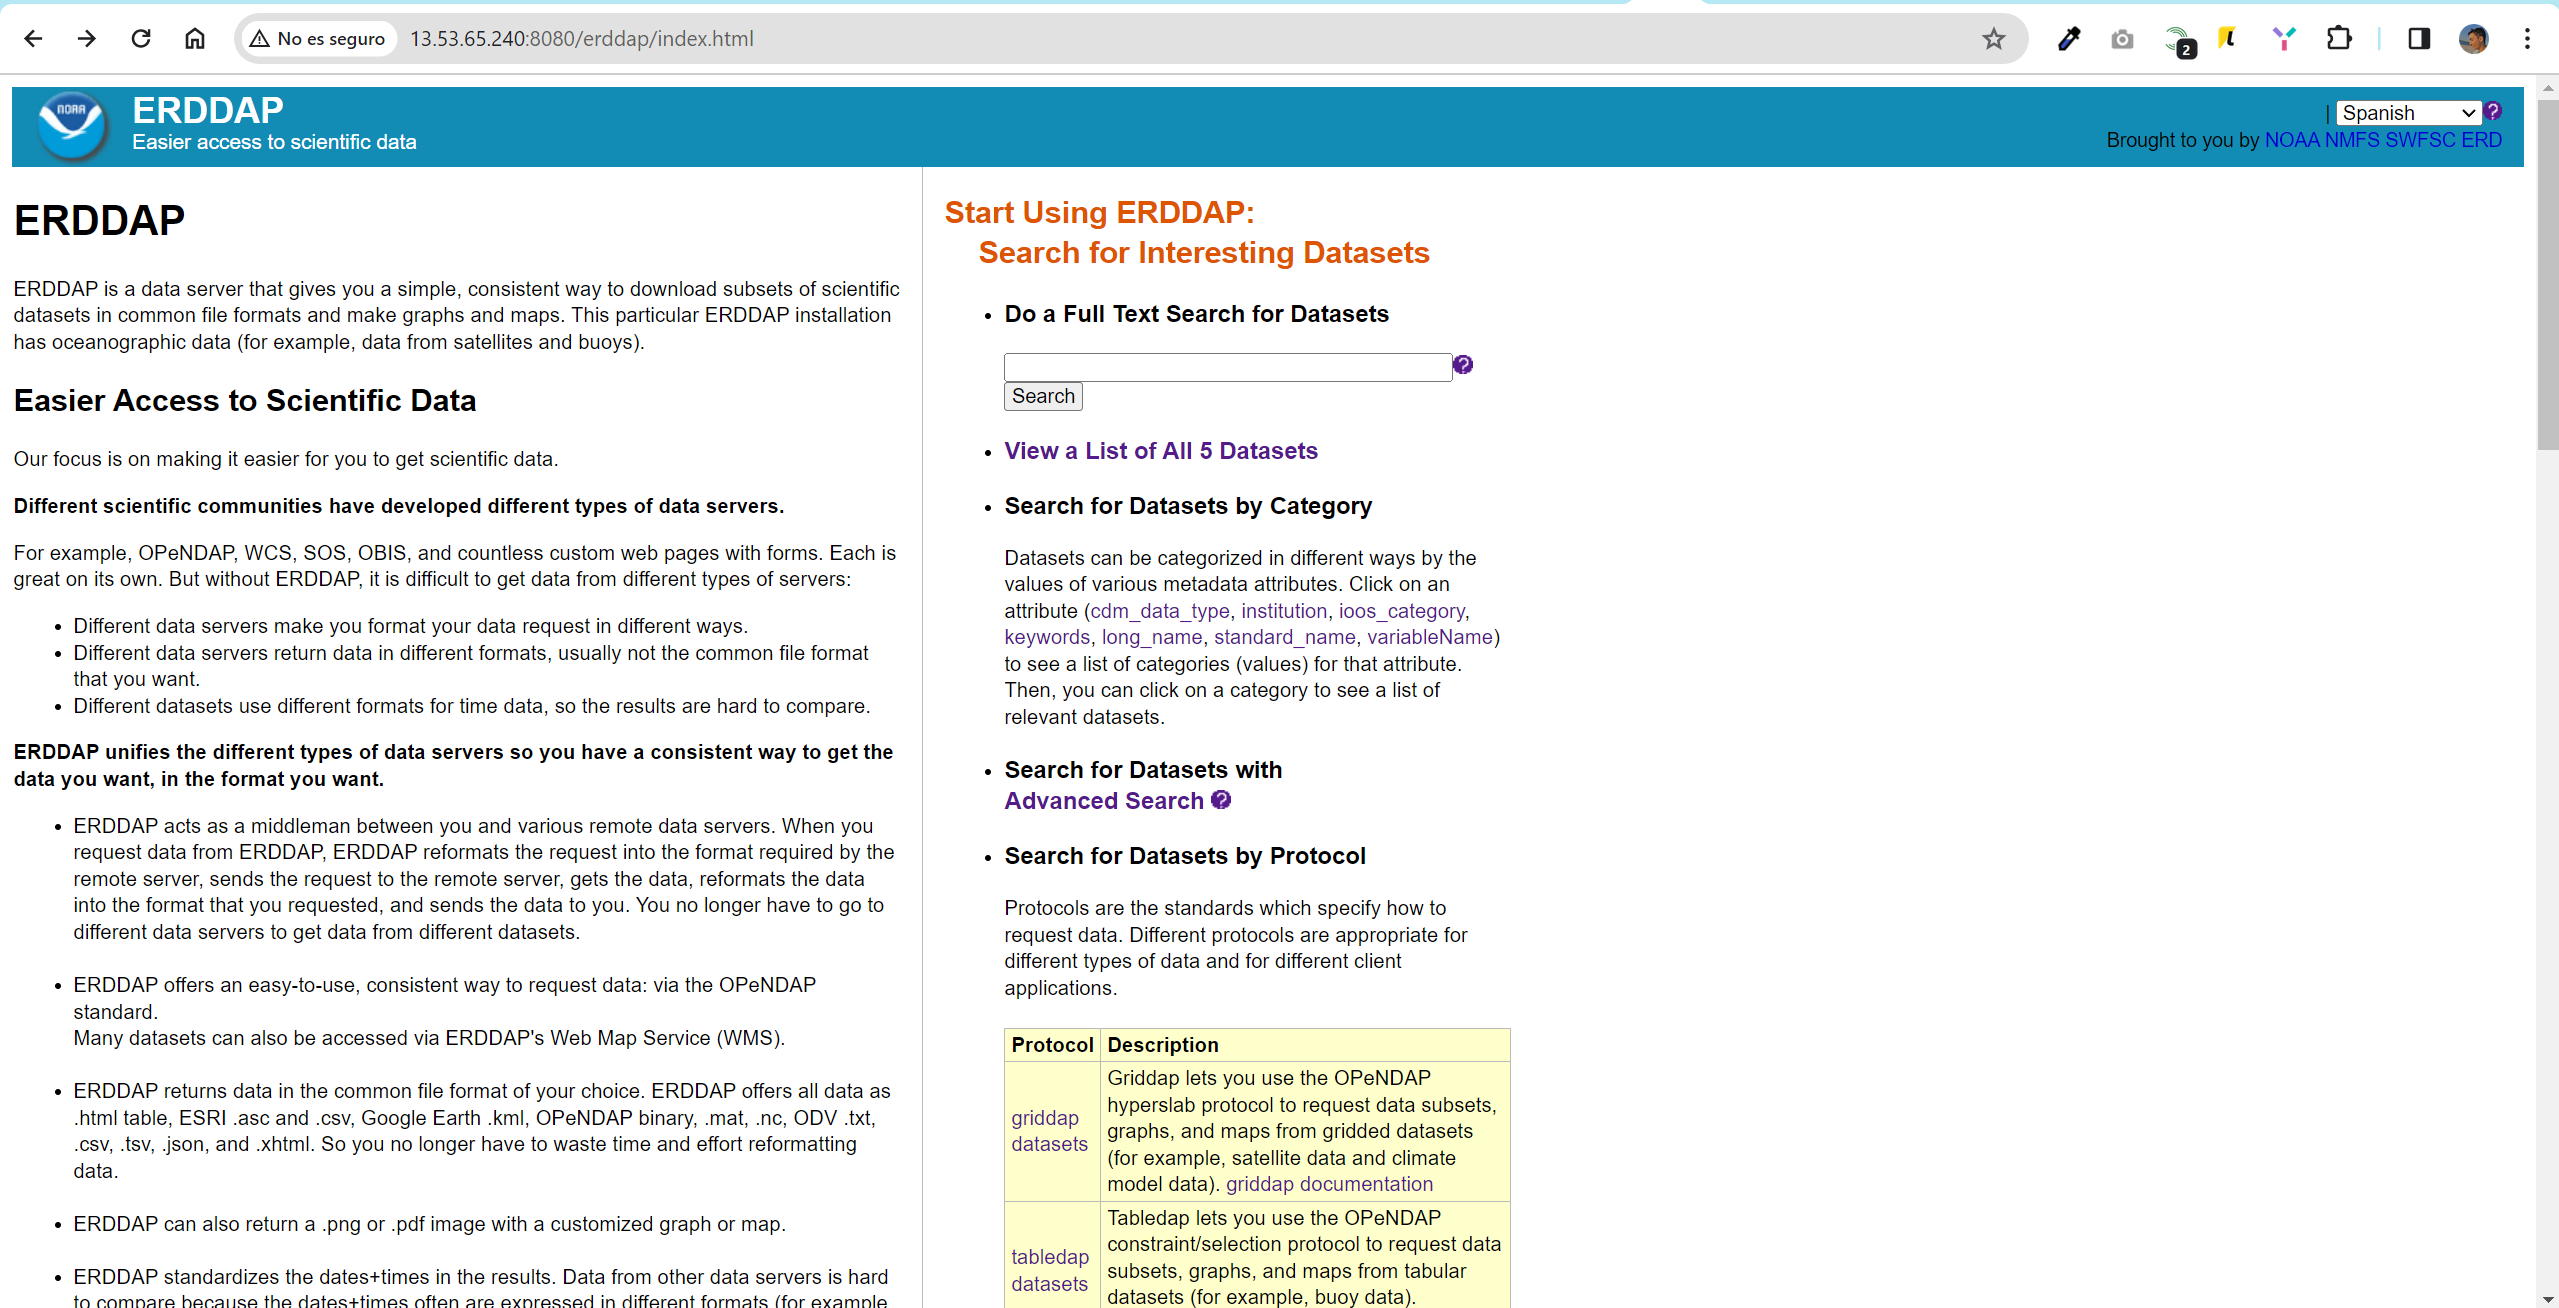
\includegraphics[width=10cm]{figuras/erddap.png}}
    \caption{Exemplo de pantalla de inicio de ERDDAP.}
    \label{fig:erddap}
\end{figure}

\begin{figure}
    \centerline{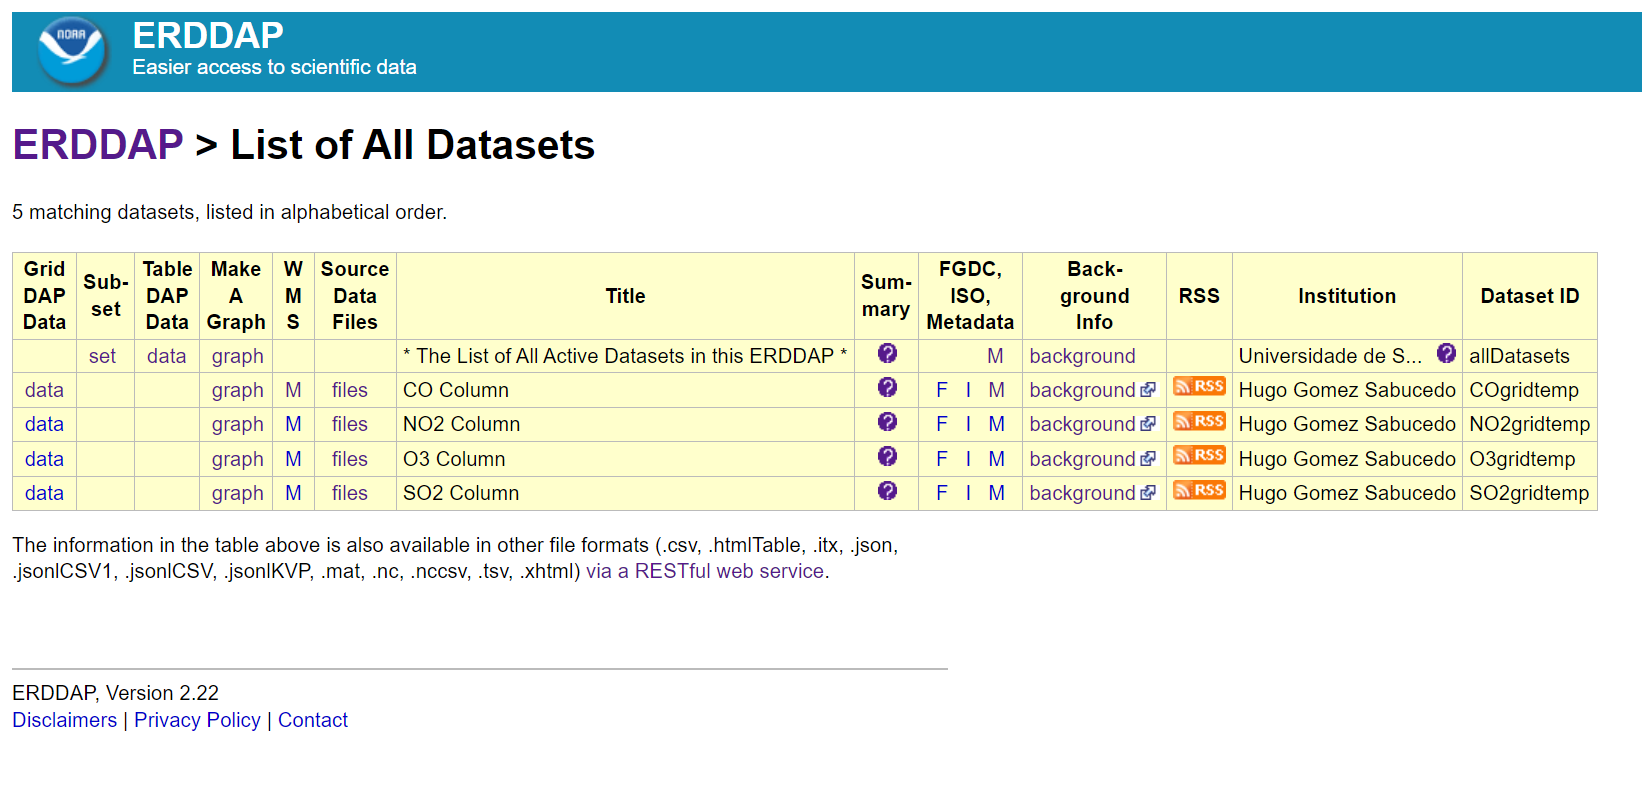
\includegraphics[width=10cm]{figuras/datasets.png}}
    \caption{Exemplo da lista de datasets dispoñibles.}
    \label{fig:listaDatasets}
\end{figure}

\begin{figure}
    \centerline{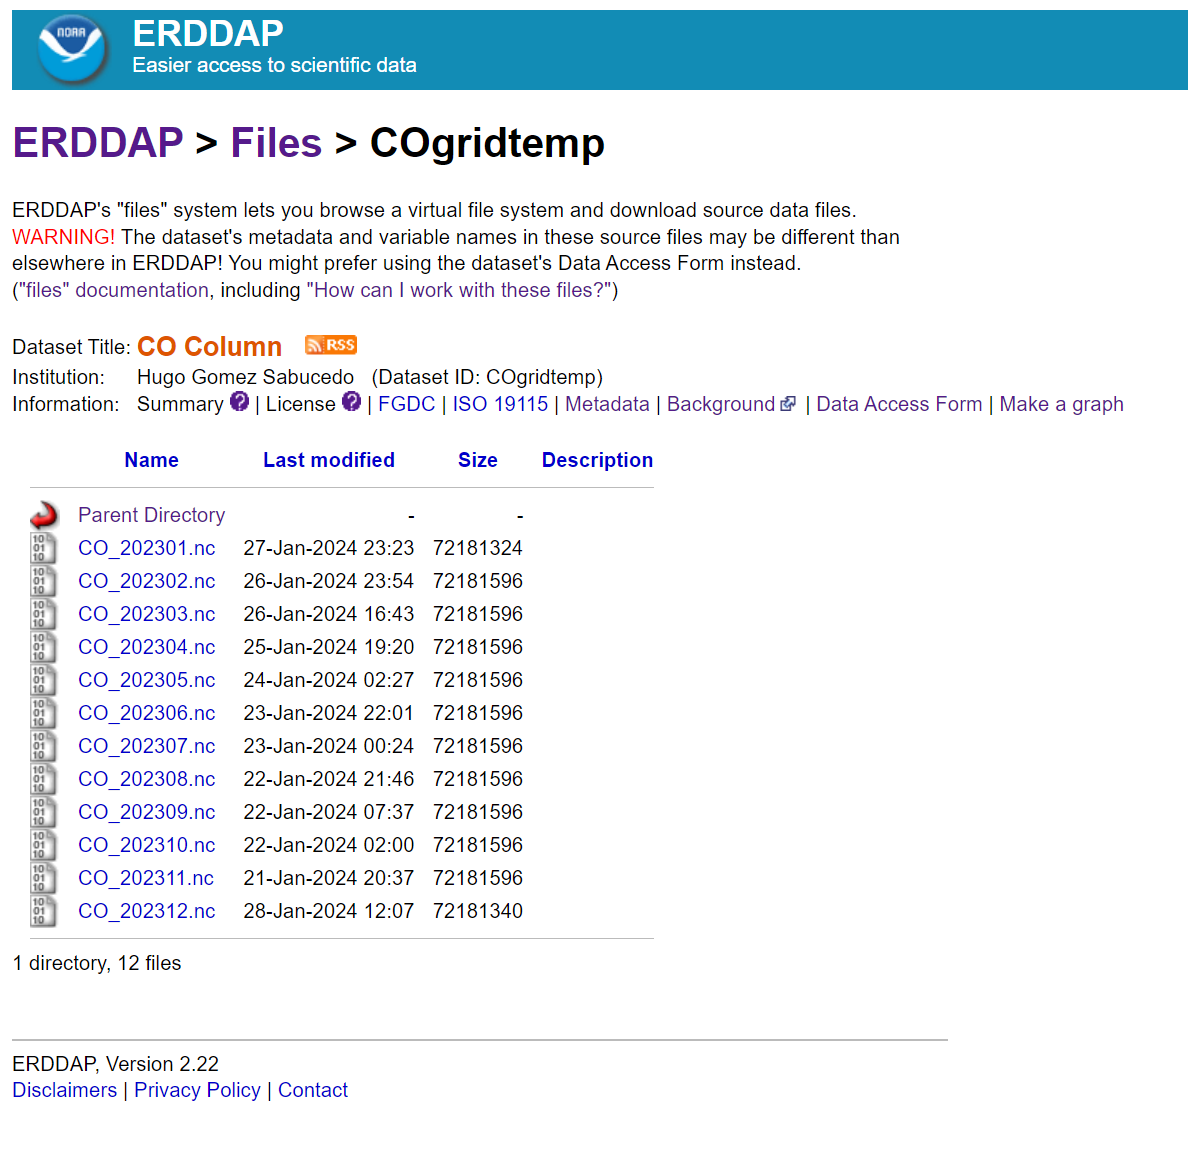
\includegraphics[width=10cm]{figuras/exemploDataset.png}}
    \caption{Exemplo da información e arquivos dun dataset.}
    \label{fig:datasetCO}
\end{figure}

Por último, comprobamos o correcto funcionamento da interface web, accesible en \url{http://13.53.65.240:8080/TROPOMIVisor/}. Ó acceder á mesma, vemos a pantalla da figura \ref{fig:interfaz}, e
podemos seleccionar, por unha parte, o parámetro para o que queremos consultar os datos e, por outra, o mes e ano. No caso de que elixamos un mes que non está dispoñible (por exemplo, febreiro de
2024), amosarase a mensaxe de error que se ve na figura \ref{fig:interfazError}.

Con todas estas probas, puidemos validar o cumprimento dos requisitos funcionais \hyperref[rf1]{[RF1]}, \hyperref[rf2]{[RF2]} e \hyperref[rf3]{[RF3]}.

\begin{figure}
    \centerline{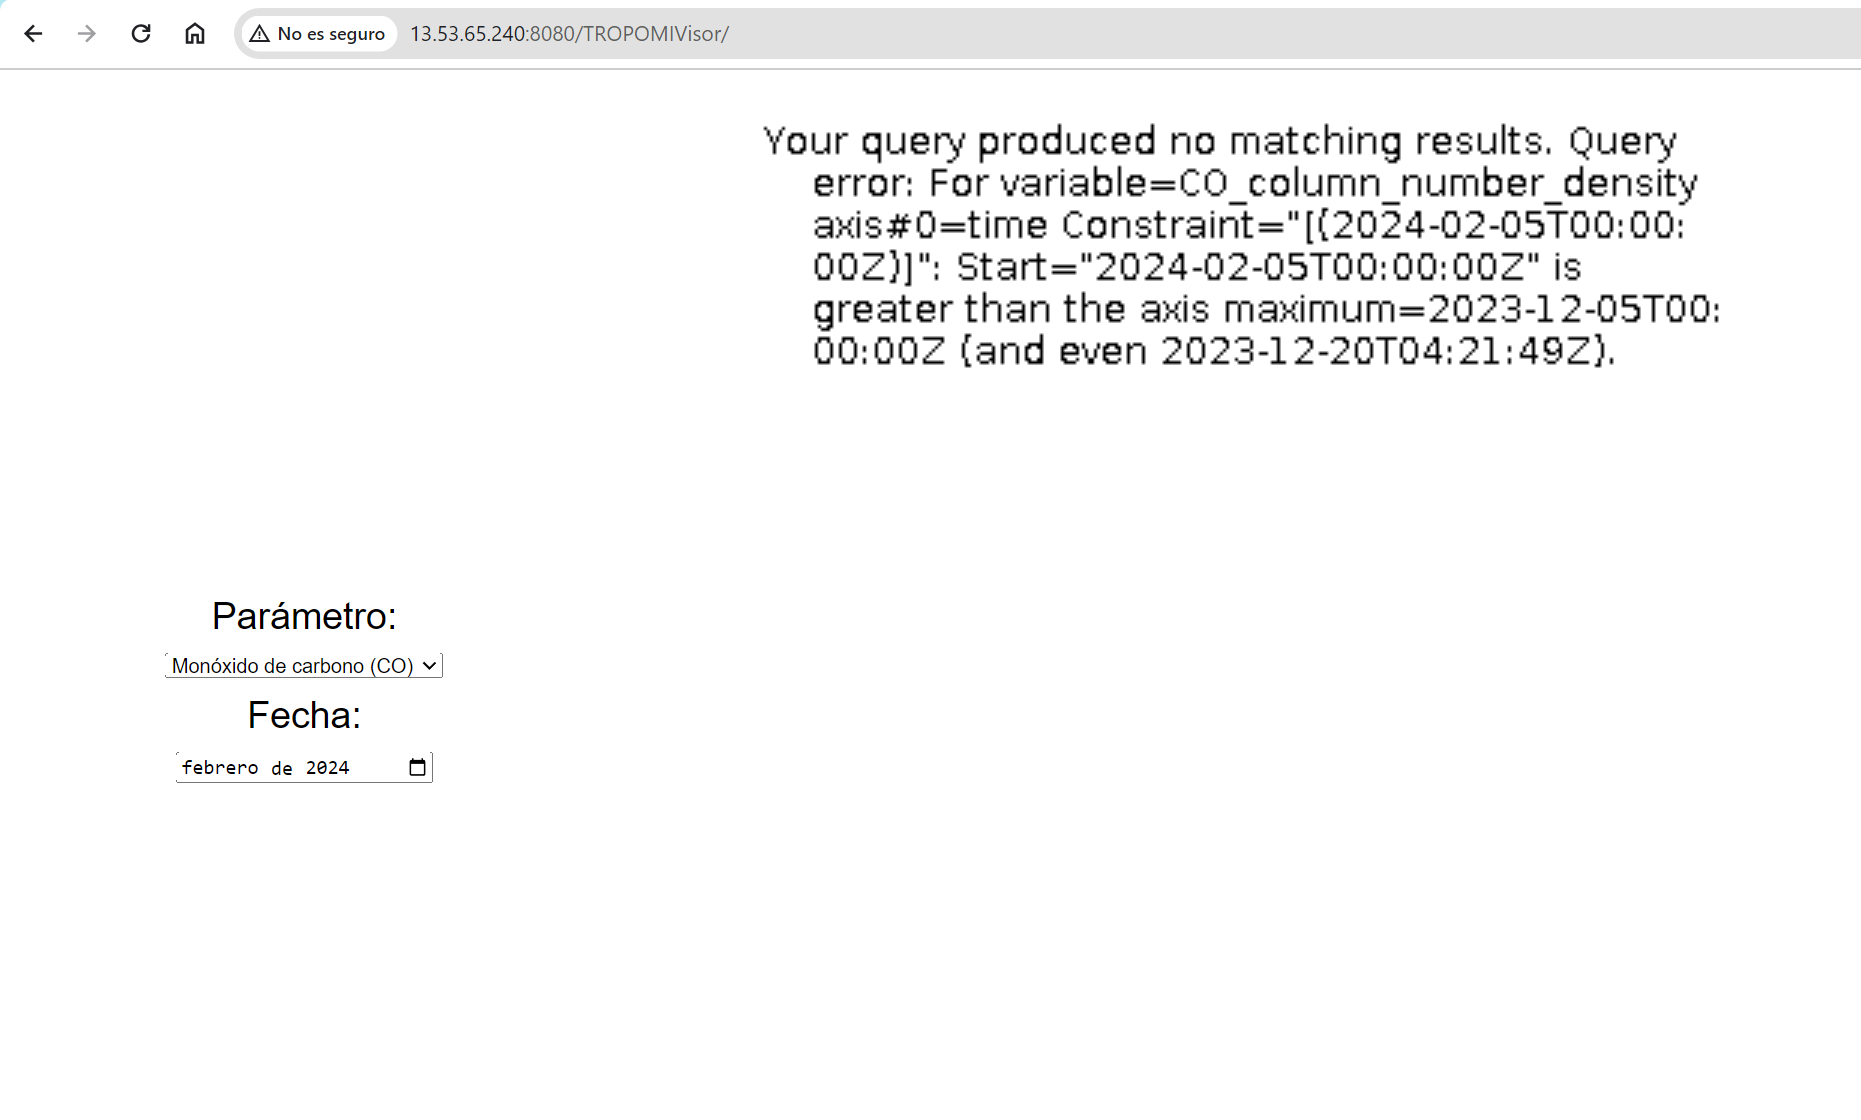
\includegraphics[width=10cm]{figuras/interfazError.png}}
    \caption{Exemplo da mensaxe de erro que se amosa na interface se introducimos un mes non dispoñible.}
    \label{fig:interfazError}
\end{figure}

\section{Probas de integración}\label{integracion}
Tamén se realizaron probas de integración da aplicación, comprobando o correcto fluxo da mesma, e asegurando que os datos se descargan, procesan e almacenan correctamente, puidendo ser visualizos
posteriormente dende a interface. Tamén se comprobou que os cambios nos datasets se reflexaran correctamente. Ademais, comprobouse o correcto funcionamento da interface de usuario, revisando a
correcta actualización dos gráficos ante un cambio na selección dos parámetros por parte do usuario.

\section{Probas de rendemento}\label{rendemento}
Por último, realizáronse probas xerais de rendemento, co obxectivo de validar o cumprimento dos requisitos non funcionais \hyperref[rnf1]{[RNF1]} e \hyperref[rnf3]{[RNF3]}. Así, validouse que a
aplicación se execute razoablemente rápido no que a descarga e procesamento de datos se refire. Se ben a descarga dos datos require unha cantidade de tempo elevada, isto é o agardable, posto que
estamos a descargar aproximadamente 50GB de datos por produto, o cal non é algo inmediato. O posterior procesamento dos datos si que é moito máis rápido, polo que podemos considerar que se cumple o
requisito de rapidez e eficiencia na aplicación, así coma o do tempo de resposta razoable.

Para verificar o requisito \hyperref[rnf2]{[RNF2]}, podemos ver canto ocupan finalmente os directorios onde se almacenan os diferentes arquivos agregados. Así, podemos ver que, para cada un dos parámetros,
o seu directorio correspondente ocupa arredor de 800MB, o cal, tratándose dos datos de todo un ano, é bastante razoable. Podemos dar por cumplido tamén o requisito de eficiencia no almacenamento.